\documentclass[12pt,a4paper]{article}

\usepackage[utf8]{inputenc}
\usepackage[T1]{fontenc}
\usepackage{lmodern}
\usepackage[brazilian]{babel}
\usepackage[margin=2.5cm]{geometry}
\usepackage{graphicx}
\usepackage{booktabs}
\usepackage{array}
\newcolumntype{L}[1]{>{\raggedright\arraybackslash}p{#1}}
\usepackage{float}
\usepackage[section]{placeins}
\usepackage{url}
\usepackage{indentfirst}
\usepackage{xcolor}
\usepackage{caption}
\usepackage{listings}
\usepackage[hidelinks]{hyperref}

\graphicspath{{diagramas/}}

\renewcommand{\topfraction}{0.85}
\renewcommand{\textfraction}{0.1}
\renewcommand{\floatpagefraction}{0.75}

\renewcommand{\lstlistingname}{Código}
\renewcommand{\lstlistlistingname}{Lista de códigos}

\lstset{
  language=Java,
  basicstyle=\ttfamily\footnotesize,
  keywordstyle=\color{blue!60!black}\bfseries,
  stringstyle=\color{green!40!black},
  commentstyle=\color{gray},
  frame=single,
  rulecolor=\color{gray!50},
  breaklines=true,
  showstringspaces=false,
  columns=fullflexible,
  keepspaces=true,
  captionpos=b,
  literate=
    {á}{{\'a}}1 {à}{{\`a}}1 {â}{{\^a}}1 {ã}{{\~a}}1
    {é}{{\'e}}1 {ê}{{\^e}}1 {í}{{\'i}}1
    {ó}{{\'o}}1 {ô}{{\^o}}1 {õ}{{\~o}}1 {ú}{{\'u}}1
    {ç}{{\c{c}}}1 {Á}{{\'A}}1 {É}{{\'E}}1 {Ç}{{\c{C}}}1
}


\title{\textbf{Sistema de Vagas do Shopping}\\[4pt]
\large Descrição Arquitetural --- Parte 1: os padrões de software}
\author{Grupo 4: [PREENCHER: integrantes]}
\date{Arquitetura e Padrões de Software --- 2026.2 --- [PREENCHER: turma]\\
Professor(a): [PREENCHER]\\[4pt]
Novembro de 2026}

\begin{document}
\maketitle

\begin{abstract}
Este documento descreve os padrões de software usados no sistema de gerenciamento das vagas de estacionamento de um shopping e explica por que cada um foi escolhido. O sistema segue o padrão arquitetural \emph{Blackboard} (memória compartilhada): um quadro central guarda o estado das vagas e o histórico de uso, e três especialistas independentes (os setores Externo e Subsolo e os relatórios gerenciais) leem e escrevem nesse quadro sem se comunicarem diretamente. Sobre essa base, o código usa quatro padrões de projeto: \emph{Singleton}, \emph{Observer}, \emph{Template Method} e \emph{Facade}. Para cada um, o texto apresenta o problema que ele resolve no sistema, o recorte do diagrama de classes, um trecho do código e as consequências. O documento também registra os padrões considerados e descartados (\emph{Strategy}, \emph{State}, \emph{Command} e \emph{Mediator}) e as regras de arquitetura que o teste automatizado confere.
\end{abstract}

\section{Introdução}

Um \textbf{padrão arquitetural} descreve a organização geral de um sistema: quais são os seus grandes componentes, qual a responsabilidade de cada um e como eles se comunicam~\cite{buschmann1996,shaw1996}. Um \textbf{padrão de projeto} atua numa escala menor: resolve um problema recorrente entre poucas classes, dentro de um componente~\cite{gamma1994}. Neste trabalho, o padrão arquitetural foi dado pelo enunciado (Blackboard), e os padrões de projeto foram escolhidos para resolver problemas concretos que apareceram ao implementá-lo.

O sistema controla dois setores de estacionamento. O \textbf{Externo} tem 15 vagas comuns (A1 a C5). O \textbf{Subsolo} tem 10 vagas (A1 a B5), aceita veículos com até 2,10~m de altura e reserva as vagas A1 e A2 como preferenciais, que exigem um motivo de uso (por exemplo, pessoa idosa ou com deficiência). Cada passagem de um veículo gera quatro eventos separados: a \emph{entrada} na cancela do setor, a \emph{ocupação} de uma vaga, a \emph{desocupação} da vaga e a \emph{saída} pela cancela. Um terceiro especialista produz onze relatórios gerenciais a partir do histórico.

O código é Java puro, sem bibliotecas externas, com duas interfaces: uma janela (Swing) e uma interface de texto. Os eventos aceitos ficam gravados num arquivo CSV e são relidos quando o programa abre.

A Tabela~\ref{tab:resumo} resume os padrões e onde cada um aparece no código.

\begin{table}[htbp]
\centering
\caption{Os padrões usados e onde aparecem no código.}
\label{tab:resumo}
\begin{tabular}{L{3.2cm}L{5.6cm}L{5.6cm}}
\toprule
\textbf{Padrão} & \textbf{Onde aparece} & \textbf{Problema que resolve} \\
\midrule
Blackboard (arquitetural) & \texttt{Blackboard}, \texttt{BlackboardController} e os especialistas em \texttt{knowledge\_sources} & Especialistas independentes cooperam por dados compartilhados, sem chamadas entre si \\
Singleton & \texttt{Blackboard} & Garantir um único quadro compartilhado \\
Observer & \texttt{Blackboard} avisa \texttt{JanelaPrincipal}, \texttt{Display} e \texttt{RegistroDeEventos} & Atualizar a tela e o arquivo sem que o quadro conheça quem os usa \\
Template Method & \texttt{KnowledgeSource.run()} e os ganchos de \texttt{EspecialistaDeSetor} & Fixar o ciclo ``condição, depois ação'' e as regras comuns aos setores \\
Facade & \texttt{FachadaEstacionamento} & Um ponto de entrada único para a janela, a interface de texto e a releitura do CSV \\
\bottomrule
\end{tabular}
\end{table}

\section{O padrão arquitetural Blackboard}

\subsection{O que é}

O padrão Blackboard nasceu em sistemas de inteligência artificial que resolviam problemas sem um algoritmo determinístico conhecido, como o reconhecimento de fala~\cite{nii1986}. A metáfora é a de especialistas diante de um quadro-negro: cada um observa o quadro, contribui quando tem algo a acrescentar e escreve o resultado para os outros verem. Nenhum especialista conversa diretamente com outro. Buschmann et al.~\cite{buschmann1996} descrevem três componentes:

\begin{itemize}
  \item o \textbf{quadro} (\emph{blackboard}), a memória central com os dados do problema e as soluções parciais;
  \item as \textbf{fontes de conhecimento} (\emph{knowledge sources}), módulos independentes, cada um com uma parte do conhecimento; cada fonte diz quando pode contribuir (a sua \emph{condição}) e o que faz (a sua \emph{ação});
  \item o \textbf{controle}, que observa o quadro e decide qual fonte de conhecimento age a seguir.
\end{itemize}

\subsection{Como aparece no código}

A Figura~\ref{fig:visao-geral} mostra as classes por pacote. A correspondência com os três componentes é direta:

\begin{itemize}
  \item \textbf{Quadro:} a classe \texttt{Blackboard} guarda as 25 vagas, a lista de estadias (cada passagem de um veículo por um setor, com as suas ocupações), a requisição pendente e o último resultado ou relatório publicado.
  \item \textbf{Fontes de conhecimento:} \texttt{ExternoKS} e \texttt{SubsoloKS} conhecem as regras de cada setor; \texttt{RelatorioKS} sabe calcular os relatórios gerenciais. Cada uma tem uma \texttt{condition()} (``esta requisição é comigo?'') e um \texttt{execute()}.
  \item \textbf{Controle:} o \texttt{BlackboardController} percorre a lista de especialistas a cada requisição, ativa o primeiro cuja condição é verdadeira e, ao fim, consome a requisição. Se nenhum especialista se candidata, ele mesmo publica a recusa ``Nenhum especialista apto''.
\end{itemize}

\begin{figure}[htbp]
\centering
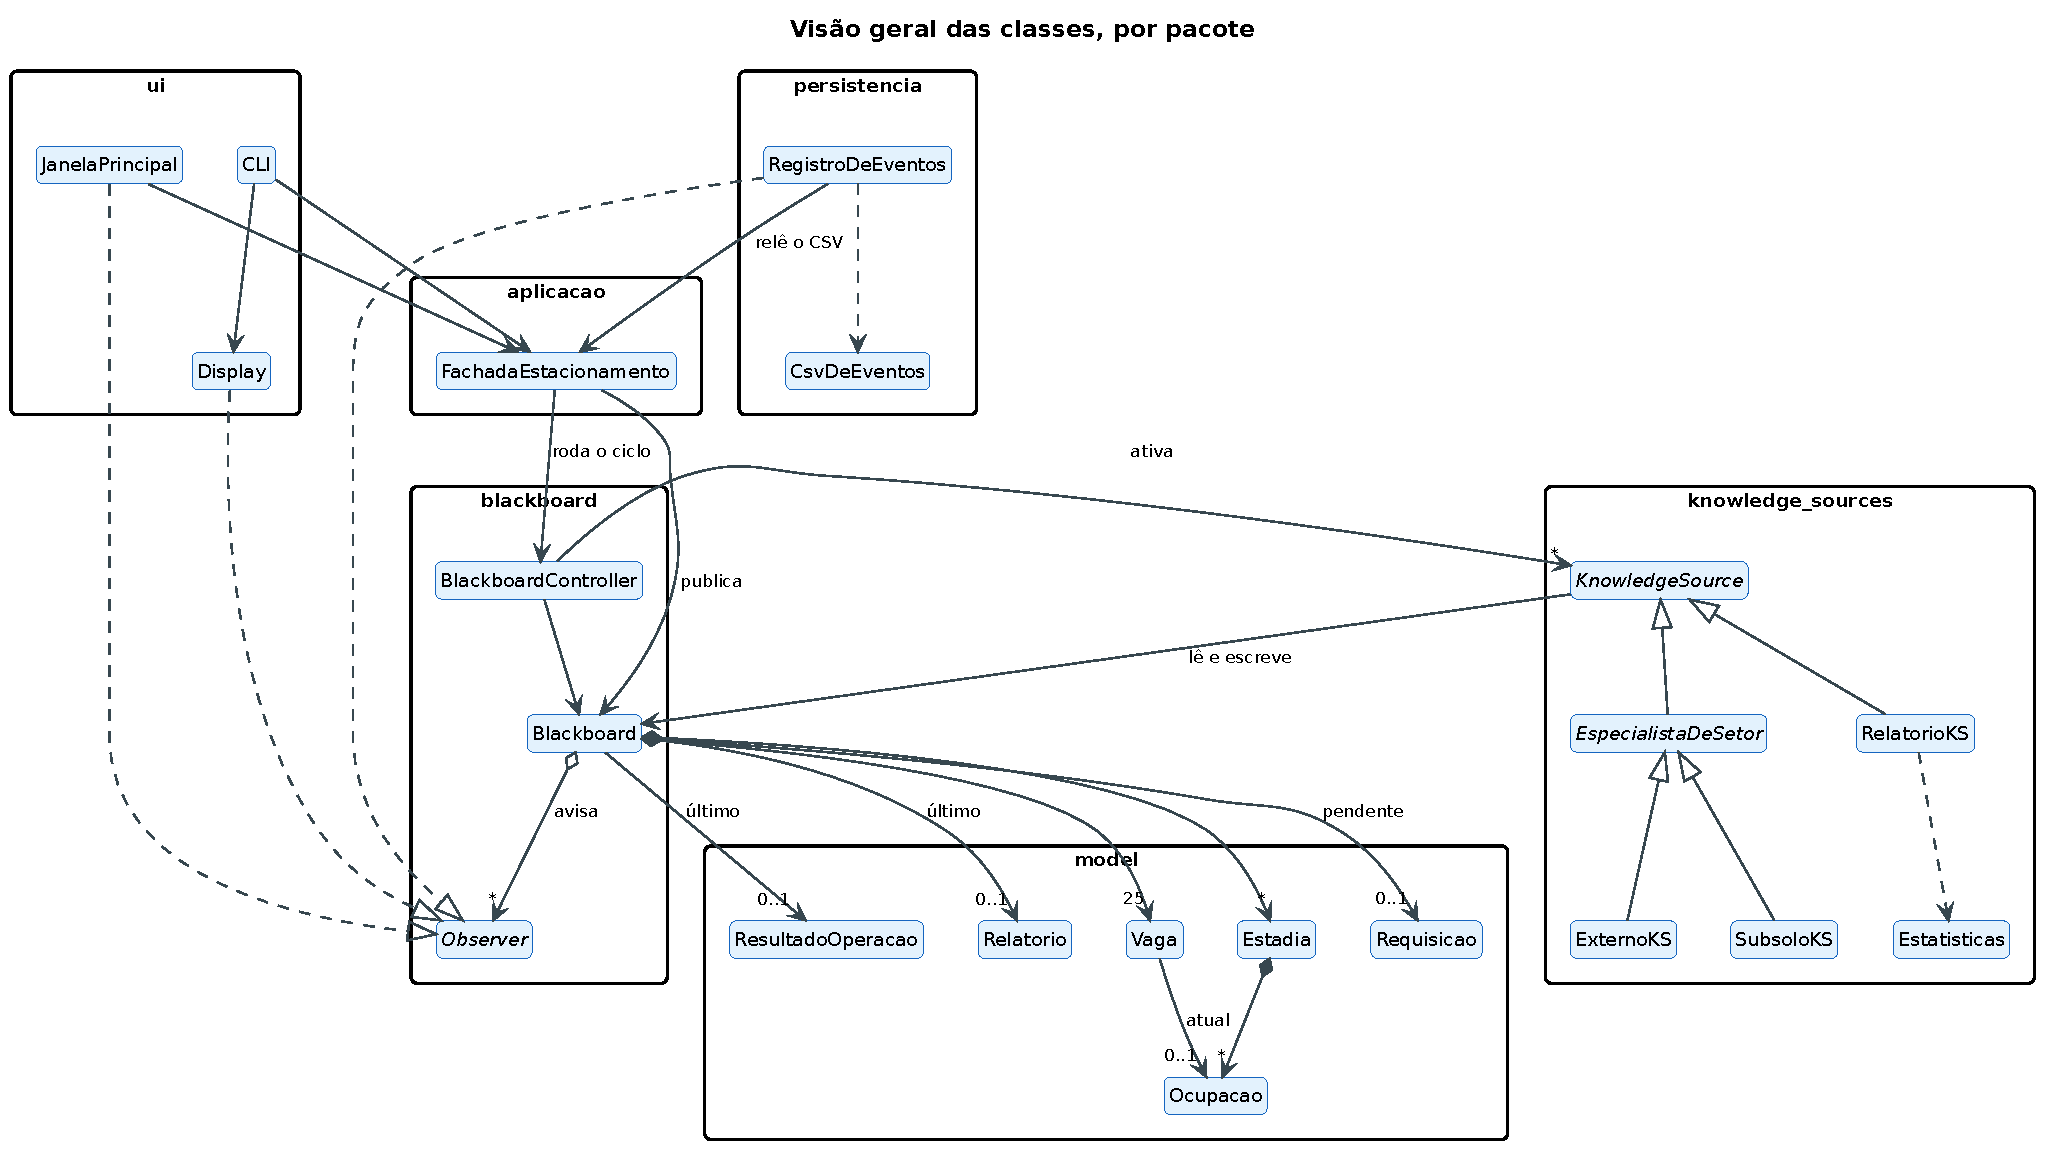
\includegraphics[width=\textwidth]{classes-visao-geral.pdf}
\caption{Visão geral das classes, por pacote.}
\label{fig:visao-geral}
\end{figure}

Um ciclo completo funciona assim. A interface monta uma \texttt{Requisicao} (por exemplo, ``ocupar a vaga A3 do Subsolo com o veículo ABC1D23'') e a entrega à fachada, que a publica no quadro e aciona o controle. O controle pergunta a cada especialista se a requisição é com ele; o \texttt{SubsoloKS} responde que sim, confere as regras lendo o quadro (o veículo entrou neste setor? a vaga existe e está livre? o horário está em ordem?) e escreve o novo estado, ou publica uma recusa com o motivo, sem alterar nada. O quadro avisa os interessados, e o controle consome a requisição. Os diagramas de atividades entregues junto com este documento detalham cada fluxo.

\subsection{Por que ele serve a este problema}

\begin{itemize}
  \item \textbf{O enunciado pede especialistas independentes.} Os setores e os relatórios não podem conversar diretamente. No Blackboard, isso não é uma disciplina que depende do cuidado de quem programa: os especialistas só conhecem o quadro, e o teste automatizado confere que nenhum deles cita outro (Seção~\ref{sec:regras}).
  \item \textbf{Os dados são o ponto de encontro natural.} O relatório de giro por vaga, por exemplo, depende das ocupações que os dois setores registraram. Como tudo está no quadro, o \texttt{RelatorioKS} lê as estadias sem perguntar nada a \texttt{ExternoKS} ou \texttt{SubsoloKS}.
  \item \textbf{Novos especialistas entram sem mexer nos existentes.} Um terceiro setor seria uma nova subclasse de \texttt{EspecialistaDeSetor} adicionada à lista do controle; nenhum especialista atual muda.
\end{itemize}

\subsection{O que ele custa}

\begin{itemize}
  \item \textbf{O quadro concentra o estado.} Toda leitura e escrita passa pela mesma classe. Por isso os métodos do \texttt{Blackboard} são \texttt{synchronized}: um aviso de tela e uma requisição nova não podem ler o quadro pela metade.
  \item \textbf{O fluxo é menos explícito.} Quem lê o código não vê uma chamada ``a janela chama o especialista do Subsolo''; vê a requisição ir ao quadro e o controle escolher quem age. Os diagramas de atividades e o painel ``Ciclo do Blackboard'' da janela, que mostra qual especialista respondeu a cada requisição, compensam essa perda de clareza.
  \item \textbf{O controle aqui é simples.} Em sistemas clássicos de Blackboard, o controle escolhe entre vários especialistas candidatos com base em prioridades. Neste sistema, cada requisição tem exatamente um especialista apto, e o controle escolhe o primeiro que se candidata. A arquitetura permite um controle mais elaborado, mas o problema não o exige.
\end{itemize}

\section{Os padrões de projeto usados}

\subsection{Singleton no Blackboard}

\paragraph{Problema.} Todos os especialistas, o controle, a fachada e as interfaces precisam trabalhar sobre o \emph{mesmo} quadro. Dois quadros na memória dividiriam o estado: um veículo poderia entrar num deles e não aparecer no outro.

\paragraph{Solução.} O Singleton~\cite{gamma1994} garante uma única instância de uma classe e oferece um ponto de acesso a ela. No \texttt{Blackboard}, o construtor é privado e o método estático \texttt{getInstance()} cria a instância na primeira chamada e a devolve nas seguintes (Código~\ref{cod:singleton}). O método é \texttt{synchronized} para que duas \emph{threads} não criem duas instâncias ao mesmo tempo, o que importa porque a janela Swing tem a sua própria \emph{thread} de desenho.

\begin{lstlisting}[caption={O ponto de acesso do Singleton (\texttt{Blackboard.java}).},label=cod:singleton]
private static Blackboard instancia;

private Blackboard() {
    popularVagas();
}

public static synchronized Blackboard getInstance() {
    if (instancia == null) {
        instancia = new Blackboard();
    }
    return instancia;
}
\end{lstlisting}

\paragraph{Consequências.} O Singleton é conhecido por dificultar os testes, porque cria um estado global que passa de um teste para o outro. Dois cuidados reduzem esse custo:

\begin{itemize}
  \item \textbf{Só o ponto de montagem chama \texttt{getInstance()}.} A classe \texttt{Main} obtém o quadro uma vez e o entrega pelo construtor aos especialistas, ao controle, à fachada e às interfaces. Nenhuma dessas classes busca o quadro por conta própria, então todas podem ser testadas com o quadro que o teste preparar.
  \item \textbf{O método \texttt{reiniciar()}} devolve o quadro ao estado inicial (todas as vagas livres e nenhuma estadia). O teste o chama entre os cenários, e a janela o usa nas opções ``Carregar cenário'' e ``Zerar dados''.
\end{itemize}

\paragraph{Alternativa recusada.} Criar o quadro com \texttt{new} no \texttt{Main} e repassá-lo resolveria o compartilhamento sem o Singleton. A escolha pelo Singleton foi mantida porque o código original do grupo já o usava, o teste confere essa propriedade (``Singleton devolve sempre a mesma instância'') e a passagem pelo construtor já elimina o principal custo do padrão.

\subsection{Observer entre o quadro e quem mostra ou grava os dados}

\paragraph{Problema.} Quando um especialista muda o quadro, três partes precisam saber: a janela, que redesenha o mapa de vagas; a interface de texto, que imprime o resultado; e o registro de eventos, que grava o evento aceito no arquivo CSV. Se o quadro chamasse essas classes diretamente, ele passaria a depender da interface gráfica e do arquivo, e cada nova forma de exibir os dados exigiria mudar o quadro.

\paragraph{Solução.} No Observer~\cite{gamma1994}, um objeto (o \emph{sujeito}) mantém uma lista de observadores e os avisa quando muda, conhecendo apenas uma interface comum a todos. Aqui o \texttt{Blackboard} é o sujeito, e a interface \texttt{Observer} tem um único método, \texttt{atualizar()} (Figura~\ref{fig:observer}). O aviso não leva dados: cada observador consulta o quadro e pega o que lhe interessa (o modelo de ``puxar'' os dados, em vez de ``empurrá-los''). A janela lê o último resultado e redesenha os mapas; o registro de eventos lê o mesmo resultado e só grava se ele for um evento aceito.

\begin{figure}[htbp]
\centering
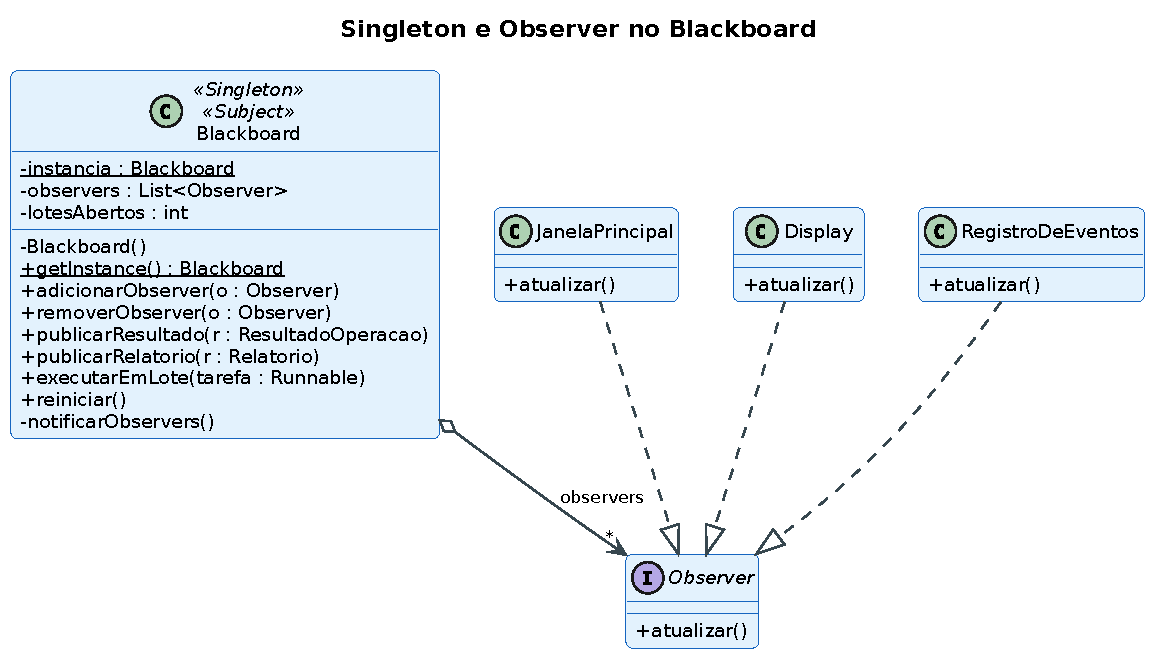
\includegraphics[width=\textwidth]{classes-singleton-observer.pdf}
\caption{Singleton e Observer no \texttt{Blackboard}.}
\label{fig:observer}
\end{figure}

O Código~\ref{cod:observer} mostra dois detalhes de implementação. Primeiro, a lista de observadores é copiada dentro do bloco sincronizado, e os avisos acontecem fora dele: assim, um observador que consulta o quadro durante o aviso não fica esperando o próprio quadro liberar a trava. Segundo, o contador \texttt{lotesAbertos} permite adiar os avisos. Quando o programa abre, o registro de eventos relê o arquivo CSV (no cenário de demonstração, 2204 eventos) dentro de \texttt{executarEmLote()}; sem o lote, a janela seria redesenhada 2204 vezes. Com ele, os observadores são avisados uma vez só, no fim.

\begin{lstlisting}[caption={O aviso aos observadores e o lote (\texttt{Blackboard.java}, resumido).},label=cod:observer]
public void executarEmLote(Runnable tarefa) {
    synchronized (this) { lotesAbertos++; }
    try {
        tarefa.run();
    } finally {
        synchronized (this) { lotesAbertos--; }
    }
    notificarObservers();
}

private void notificarObservers() {
    List<Observer> copia;
    synchronized (this) {
        if (lotesAbertos > 0) return;
        copia = new ArrayList<>(observers);
    }
    for (Observer o : copia) {
        o.atualizar();
    }
}
\end{lstlisting}

\paragraph{Consequências.} O quadro não importa nenhuma classe de interface nem de persistência, e o teste confere isso. Acrescentar o registro em CSV, por exemplo, não exigiu nenhuma mudança nos especialistas: bastou uma nova classe que implementa \texttt{Observer}. O custo é que um observador precisa descobrir sozinho o que mudou. O registro de eventos guarda o último resultado que já viu, para não gravar a mesma linha duas vezes, e a janela, que pode ser avisada a partir de qualquer \emph{thread}, agenda o redesenho na \emph{thread} do Swing com \texttt{SwingUtilities.invokeLater}.

\subsection{Template Method nos especialistas}

\paragraph{Problema.} O padrão Blackboard exige que todo especialista siga o mesmo protocolo: primeiro avalia a condição; só se ela for verdadeira, executa a ação. Se cada especialista escrevesse esse protocolo, um deles poderia agir sem conferir a condição. Além disso, os dois setores têm quase as mesmas regras (entrar, ocupar, desocupar e sair funcionam igual), e o Subsolo acrescenta só duas: o limite de altura na entrada e o motivo obrigatório nas vagas preferenciais. Copiar os quatro fluxos nas duas classes duplicaria as regras.

\paragraph{Solução.} O Template Method~\cite{gamma1994} define o esqueleto de um algoritmo num método da classe-mãe e deixa alguns passos para as subclasses. O padrão aparece em dois níveis (Figura~\ref{fig:template}):

\begin{itemize}
  \item Em \texttt{KnowledgeSource}, o método \texttt{run()} é \texttt{final} e fixa o protocolo (Código~\ref{cod:run}). As subclasses implementam \texttt{condition()} e \texttt{execute()}, mas não podem mudar a ordem entre elas.
  \item Em \texttt{EspecialistaDeSetor}, a classe-mãe dos dois setores, \texttt{condition()} e \texttt{execute()} também são \texttt{final} e contêm os quatro fluxos completos. Os pontos que variam são \emph{ganchos} (\emph{hooks}): métodos com um comportamento padrão que a subclasse pode sobrescrever. \texttt{problemaNaEntrada} e \texttt{problemaNaOcupacao} devolvem \texttt{null} (``nenhum problema''); o \texttt{SubsoloKS} os sobrescreve (Código~\ref{cod:ganchos}), e o \texttt{ExternoKS} só informa qual é o seu setor.
\end{itemize}

\begin{figure}[htbp]
\centering
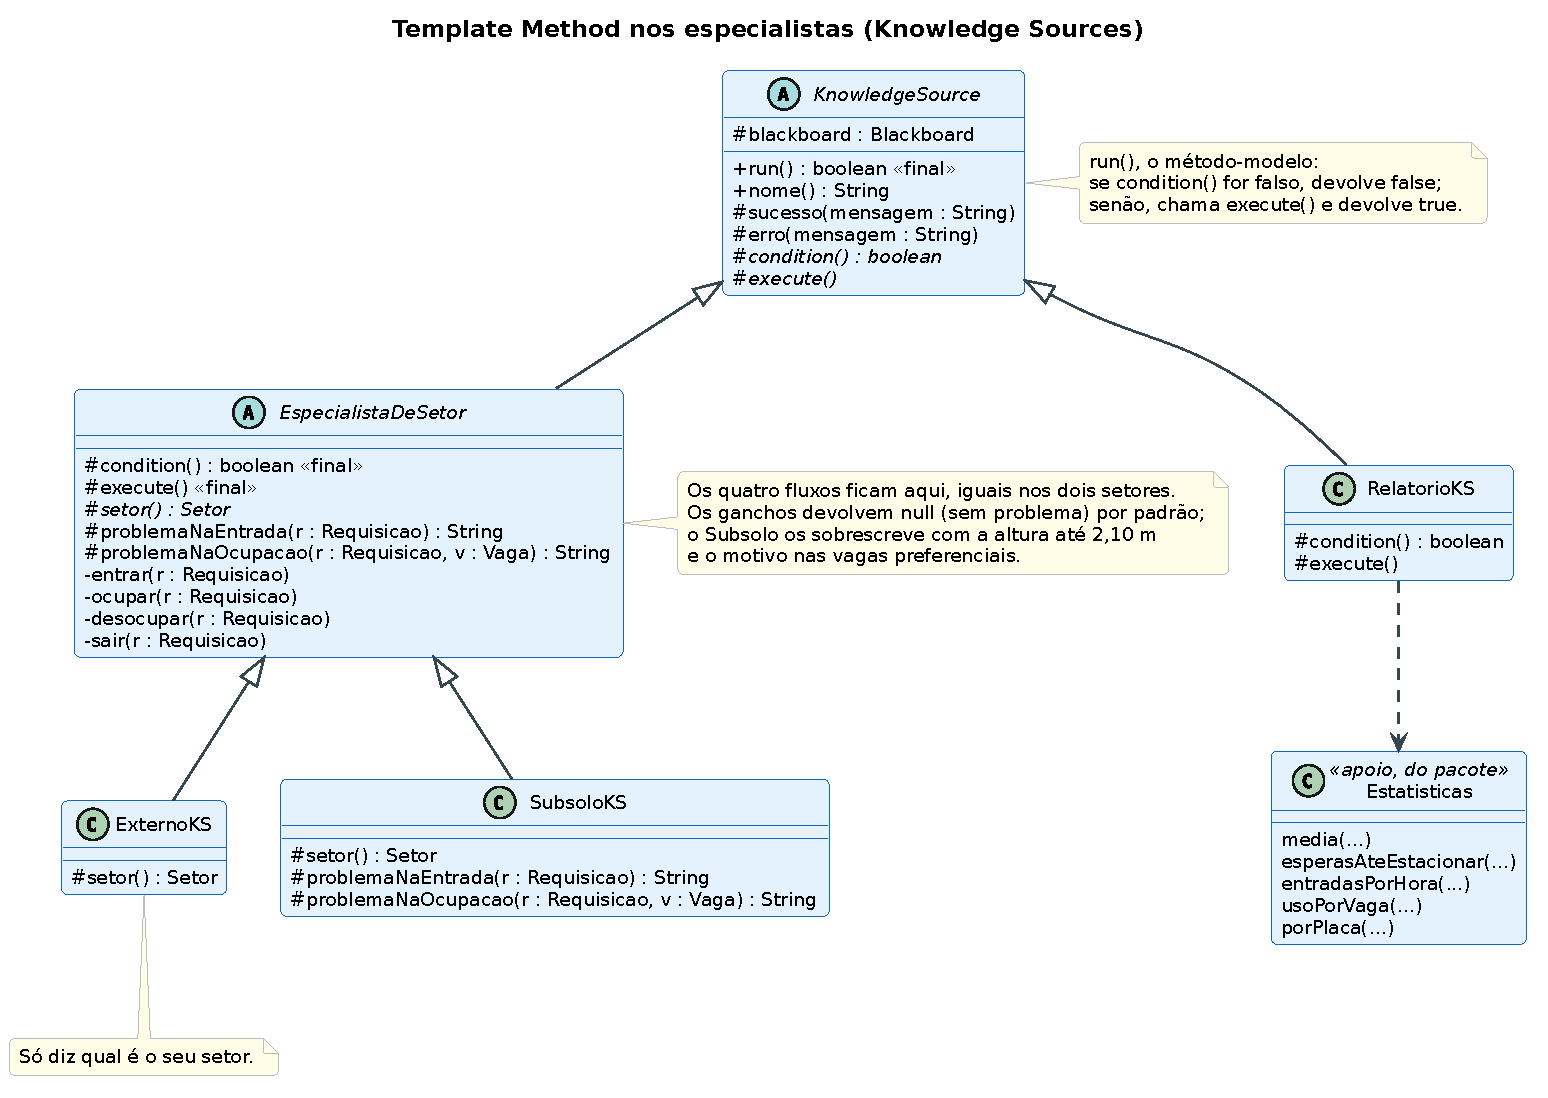
\includegraphics[width=\textwidth]{classes-template-method.pdf}
\caption{Template Method nos especialistas.}
\label{fig:template}
\end{figure}

\begin{lstlisting}[caption={O método-modelo (\texttt{KnowledgeSource.java}).},label=cod:run]
public final boolean run() {
    if (!condition()) {
        return false;
    }
    execute();
    return true;
}
\end{lstlisting}

\begin{lstlisting}[caption={Os ganchos do Subsolo (\texttt{SubsoloKS.java}, resumido).},label=cod:ganchos]
@Override
protected String problemaNaEntrada(Requisicao r) {
    Double altura = r.getAltura();
    if (altura == null) {
        return "Altura do veículo é obrigatória no Subsolo.";
    }
    if (altura > ALTURA_MAXIMA) {
        return "Veículo não permitido no Subsolo: ...";
    }
    return null;
}

@Override
protected String problemaNaOcupacao(Requisicao r, Vaga vaga) {
    if (vaga.isPreferencial() && r.getMotivo() == null) {
        return "Vaga " + vaga.getId() + " é preferencial e exige um motivo ...";
    }
    return null;
}
\end{lstlisting}

\paragraph{Consequências.} As regras comuns ficam num só lugar: a recusa de um horário fora de ordem, por exemplo, foi escrita uma vez e vale para os dois setores. A herança não cria comunicação entre os especialistas: \texttt{ExternoKS} e \texttt{SubsoloKS} compartilham \emph{código} pela classe-mãe, mas cada instância só conversa com o quadro. O custo é o acoplamento típico da herança: uma mudança em \texttt{EspecialistaDeSetor} afeta os dois setores. Isso é desejável aqui, porque as regras comuns devem mesmo mudar juntas. O \texttt{RelatorioKS} herda direto de \texttt{KnowledgeSource}, porque não trata eventos de setor.

\paragraph{Alternativa recusada.} Cada setor poderia receber as suas regras extras como objetos (composição, no estilo Strategy). Com só duas regras extras, num só setor, a classe com ganchos é mais simples de ler e mantém o protocolo protegido pelo \texttt{final}.

\subsection{Facade na entrada do sistema}

\paragraph{Problema.} Três partes do sistema enviam requisições: a janela, a interface de texto e o registro de eventos, que reenvia cada linha do CSV ao abrir o programa. Para enviar uma requisição, é preciso preencher o horário (se faltar), publicá-la no quadro, rodar o ciclo do controle e localizar o resultado daquela requisição. Repetir esses passos em três lugares espalharia o protocolo do Blackboard pelas interfaces.

\paragraph{Solução.} Uma Facade~\cite{gamma1994} oferece uma interface única e simples para um subsistema. A \texttt{FachadaEstacionamento} tem um método por operação (\texttt{entrar}, \texttt{ocupar}, \texttt{desocupar}, \texttt{sair} e \texttt{gerarRelatorio}) e o método geral \texttt{enviar}, que faz o protocolo completo (Figura~\ref{fig:facade} e Código~\ref{cod:facade}). O resultado só é devolvido se for a resposta \emph{desta} requisição; assim, um relatório aceito, que publica um relatório em vez de um resultado, não devolve por engano o resultado de uma operação anterior.

\begin{figure}[htbp]
\centering
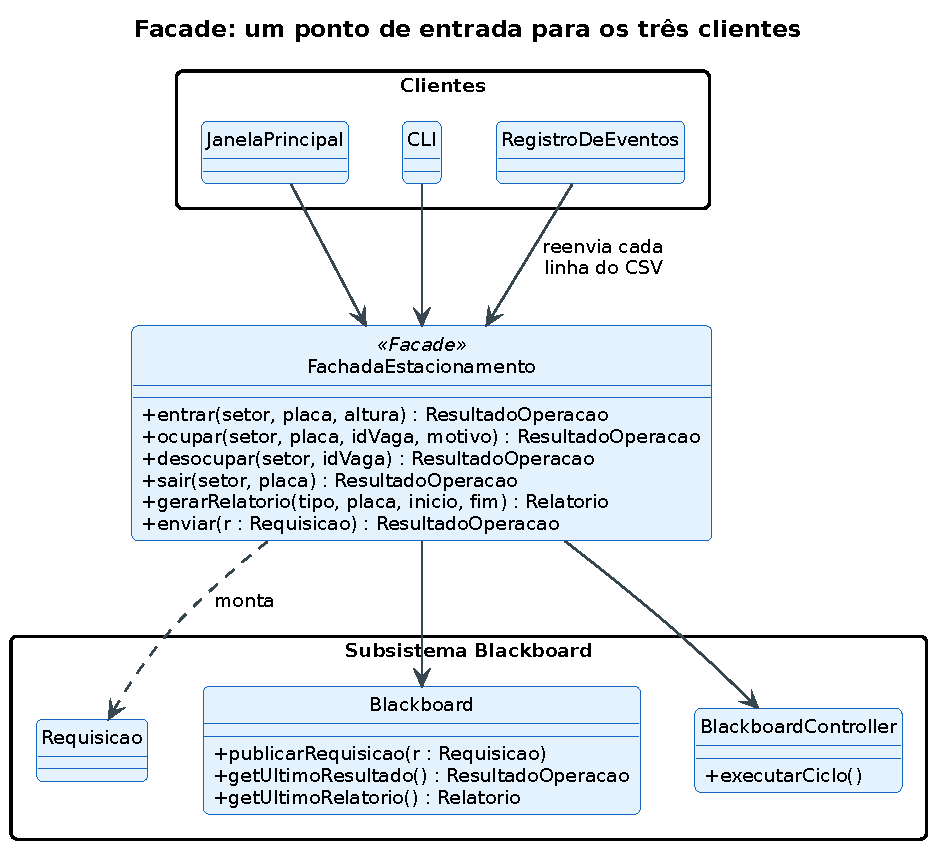
\includegraphics[width=0.85\textwidth]{classes-facade.pdf}
\caption{A fachada entre os três clientes e o subsistema Blackboard.}
\label{fig:facade}
\end{figure}

\begin{lstlisting}[caption={O protocolo encapsulado pela fachada (\texttt{FachadaEstacionamento.java}).},label=cod:facade]
public ResultadoOperacao enviar(Requisicao requisicao) {
    if (requisicao.getMomento() == null) requisicao.setMomento(LocalDateTime.now());
    blackboard.publicarRequisicao(requisicao);
    controlador.executarCiclo();
    ResultadoOperacao r = blackboard.getUltimoResultado();
    return r != null && r.getRequisicao() == requisicao ? r : null;
}
\end{lstlisting}

\paragraph{Consequências.} As interfaces não conhecem o controle (o teste confere que nenhuma delas importa o \texttt{BlackboardController} nem os especialistas) e ficam só com o que é delas: validar o \emph{formato} do que o usuário digitou e mostrar o resultado. As regras de negócio continuam todas nos especialistas. A releitura do CSV passa pelo mesmo caminho de uma operação feita na tela, e por isso cada linha relida é conferida pelas mesmas regras. A fachada não esconde o quadro por completo: as interfaces ainda o leem para desenhar o mapa, o que é coerente com o Observer, em que os observadores consultam o sujeito.

\section{Padrões considerados e descartados}

\subsection{Strategy nos relatórios}

O \texttt{RelatorioKS} escolhe entre os onze relatórios com um \texttt{switch} sobre o tipo pedido. O Strategy~\cite{gamma1994} trocaria esse \texttt{switch} por uma classe por relatório, todas com a mesma interface. A troca foi recusada por três motivos:

\begin{itemize}
  \item \textbf{O tipo de relatório é escolhido a cada pedido, não configurado.} O Strategy compensa quando um objeto é montado com um algoritmo e o usa por muito tempo. Aqui, cada requisição já traz o tipo, e o \texttt{switch} apenas despacha.
  \item \textbf{O compilador confere que todos os tipos foram tratados.} O \texttt{switch} é uma expressão do Java sem o caso \texttt{default}: se alguém acrescentar um tipo de relatório e esquecer de tratá-lo, o código não compila.
  \item \textbf{O conhecimento de relatórios fica num especialista só.} Onze classes de estratégia espalhariam esse conhecimento fora da fonte de conhecimento. Os cálculos que os relatórios dividem (médias, picos e giro, por exemplo) foram separados numa classe de apoio, \texttt{Estatisticas}, visível só dentro do pacote.
\end{itemize}

\begin{lstlisting}[caption={O despacho dos relatórios (\texttt{RelatorioKS.java}, resumido).},label=cod:switch]
Relatorio relatorio = switch (r.getTipoRelatorio()) {
    case OCUPACAO -> gerarOcupacao();
    case HISTORICO_POR_PLACA -> gerarHistoricoPorPlaca(r.getPlaca());
    // ... um caso para cada um dos onze tipos
    case COMPLETO -> gerarCompleto();
};
blackboard.publicarRelatorio(relatorio);
\end{lstlisting}

\subsection{State na vaga e no veículo}

A vaga (livre ou ocupada) e o veículo (circulando ou estacionado) têm estados bem definidos, e os diagramas de estados entregues junto com este documento os descrevem. O State~\cite{gamma1994} colocaria o comportamento de cada estado num objeto (``uma vaga livre sabe ser ocupada''). Isso contraria o Blackboard: as regras de transição são o conhecimento dos especialistas, e o quadro deve guardar dados passivos. Ocupar uma vaga, por exemplo, depende de regras que envolvem a vaga, a estadia do veículo e o setor (o veículo entrou neste setor? já ocupa outra vaga? a vaga é preferencial?); com o State, parte dessas regras iria para dentro do quadro. Além disso, os estados são calculados, e não guardados: a vaga está ocupada quando tem uma ocupação atual, e o veículo está estacionado quando a sua estadia tem uma ocupação em aberto. Assim, o mesmo fato não fica registrado em dois lugares que poderiam se contradizer.

\subsection{Command na requisição}

A \texttt{Requisicao} parece um Command~\cite{gamma1994}, porque representa um pedido como objeto. A diferença está em quem executa. No Command, o objeto sabe se executar (tem um método \texttt{execute()}) ou conhece o seu receptor. No Blackboard, a requisição é só um conjunto de dados, e quem a executa é decidido na hora pelo controle, conforme a condição dos especialistas. Transformá-la num Command fixaria o executor de antemão e anularia o controle do Blackboard. Os benefícios típicos do Command (desfazer, refazer, fila de comandos) também não são pedidos pelo enunciado.

\subsection{Por que o controle não é um Mediator}

O \texttt{BlackboardController} conhece todos os especialistas, como um Mediator~\cite{gamma1994} conhece os seus colegas. Mas, no Mediator, os colegas se comunicam \emph{por meio} do mediador: cada um o avisa de um acontecimento, e o mediador repassa a informação aos outros. Aqui, os especialistas não conhecem o controle, não lhe enviam mensagens e não recebem mensagens uns dos outros. O controle só decide \emph{quem age a seguir}; a informação circula pelos dados do quadro. Esse papel de escalonador é o componente de controle do próprio padrão Blackboard~\cite{buschmann1996}, e não um padrão de projeto separado.

\section{Regras de arquitetura conferidas pelo teste}
\label{sec:regras}

As decisões acima só se mantêm se o código continuar a respeitá-las. Por isso, o teste automatizado do projeto (\texttt{SmokeTest}, com 90 verificações) inclui verificações de estrutura e uma análise do código-fonte que falha se alguma regra for quebrada. A Tabela~\ref{tab:regras} lista as que dizem respeito aos padrões.

\begin{table}[htbp]
\centering
\caption{Verificações do teste ligadas aos padrões.}
\label{tab:regras}
\begin{tabular}{L{7.5cm}L{6.5cm}}
\toprule
\textbf{Verificação} & \textbf{O que protege} \\
\midrule
Singleton devolve sempre a mesma instância & Singleton \\
\texttt{run()} é final & Template Method \\
Setores herdam de \texttt{EspecialistaDeSetor}; relatórios não & Template Method com ganchos \\
\texttt{condition()} não tem efeito colateral e só aceita o que é seu & Protocolo do Blackboard \\
\texttt{executarEmLote()} adia as notificações e avisa uma vez no fim & Observer com lote \\
Nenhum especialista cita outro especialista & Independência dos especialistas \\
Nenhum especialista importa a interface nem usa \texttt{System.out} & Especialistas só falam com o quadro \\
O \texttt{Blackboard} não importa especialistas, fachada nem persistência & Quadro passivo; Observer \\
Fachada e persistência não importam especialistas & Facade sobre o controle \\
Interfaces não importam especialistas nem o controle & Facade \\
\texttt{System.out} só aparece no pacote \texttt{ui} & Separação entre regras e exibição \\
\bottomrule
\end{tabular}
\end{table}

\section{Conclusão}

O Blackboard organiza o sistema em torno dos dados: os especialistas dos setores e dos relatórios são independentes e cooperam só pelo quadro. Os quatro padrões de projeto resolvem problemas que essa organização cria. O Singleton garante um único quadro. O Observer avisa a tela e o arquivo sem que o quadro dependa deles. O Template Method protege o protocolo ``condição, depois ação'' e evita duplicar as regras dos setores. A Facade dá às interfaces um ponto de entrada único. Os padrões descartados foram recusados porque moveriam o conhecimento para fora dos especialistas (Strategy e State), porque fixariam o executor que o controle deve escolher (Command) ou porque descrevem uma comunicação que o sistema não tem (Mediator).

\bibliographystyle{plain}
\bibliography{referencias}

\end{document}
